\chapter{My contribution}
\label{cha:TheThesis}

Taking the existing methods as reference (see section \ref{cha:relatedWork}) a new segmentation approach is developed. Thereby, the main focus is to reduce the computation steps of the correlated correspondence algorithm \cite{CorrelatedCorrespondance} as well as the LRP algorithm \cite {guo2016correspondence}. The approach has been first implemented in 2D, in order to be able to focus solely on developing and testing. Subsequently, it will be implemented in 3D using the PCL.

\section{Goal and approach}

The goal is to segment an articulated mesh $M$ into its unknown number $n$ of rigid parts $\mathcal{P} =  \{P_1,\ldots,P_n\}$ and extract the joints $\mathcal{J} =  \{J_1,\ldots,J_m\}$ linking those parts in form of a skeleton structure. In general, this is done by non-rigid registration of the point clouds $C_{1,0}$ and $C_{2,0}$ of an object in two different poses. $C_{1,0}$ is thereby used as a \textit{template} to be registered with $C_{2,0}$. The main task is to determine a part assignment $P_i$ and the corresponding transformation $T_i$ for all points of the \textit{template} that aligns them with all points of $C_{2,0}$. Basically, a divide and conquer approach is implemented to recursively subdivide $C_{1,0}$ and $C_{2,0}$ into matching clusters. 

\section{Assumptions}

The input mesh $M$ is assumed to solely consist of rigid parts that can not be deformed or stretched (e.g. rigid parts of a human) and are linked by joints. Comparing two poses being adopted by the articulated object, the geodesic distance $g(\boldsymbol{p}_i,\boldsymbol{p}_j)$ between two mesh points $\boldsymbol{p}_i(x,y)$ and $\boldsymbol{p}_j(x,y)$ remains constant. Thereby, it is taken advantage of the knowledge that points located on a rigid part $P_i$ have the same transformation $T_i$ . Furthermore, it is assumed that the two poses of $M$ are oriented in the same direction.

\section{General approach}

The algorithm starts with two sets of point clouds $C_{1,0}$ and $C_{2,0}$ of an object $M$ in different poses (see figure \ref{fig:pc_2parts}). The two point clouds are iteratively subdivided into point clusters $\mathcal{C}_1 =  \{C_{1,1},\ldots, C_{1,m}\}$ and $\mathcal{C}_2 =  \{C_{2,1},\ldots, C_{2,m}\}$. In each iteration step two related clusters of $C_{1,0}$ and $C_{2,0}$ are verified to match by applying the ICP (iterative closest point), resulting in a matching error $e$. In case of $ e < \tau $, two clusters are assumed to match. Otherwise, the algorithm is applied recursively and the clusters are again subdivided into further clusters. The algorithm terminates if all resulting clusters of $C_{1,0}$ can be matched to all clusters of $C_{2,0}$. All neighboring clusters are then checked to be merged, in case of having divided a rigid part. After that step, the remaining clusters are assigned to rigid parts $\mathcal{P} =  \{P_1,\ldots,P_n\}$.

\subsection{Removing outliers}

As a first step, the outliers of the point clouds of $M$ are removed. This is done, by iteratively detecting point clusters $\mathcal{C} = \{C_0, \ldots , C_m\}$ from all points of $M$. A cluster $C_i$ is grown from an unclustered point $\boldsymbol{p}_i(x,y)$. Another point $\boldsymbol{p}_j(x,y)$ is added to the cluster $C_i$ if the euclidean distance between them $d(\boldsymbol{p}_i, \boldsymbol{p}_j)$ is below a pre-defined threshold $\tau$. This threshold is thereby depending on the resolution and density of $M$. All points of $C_i$ are then iteratively compared to the remaining unclustered points to allow the cluster to grow. Once, all points of $C_i$ have been treated, another unclustered point is used as a seed. If there are no unclustered points left, the clusters with the highest number of points $n$ are selected as input clusters $C_{1,0}$ and $C_{2,0}$ (see figure \ref{fig:pc_2parts}).

\begin{figure}[htbp]
	\centering\small
	\begin{tabular}{cc}
		\fbox{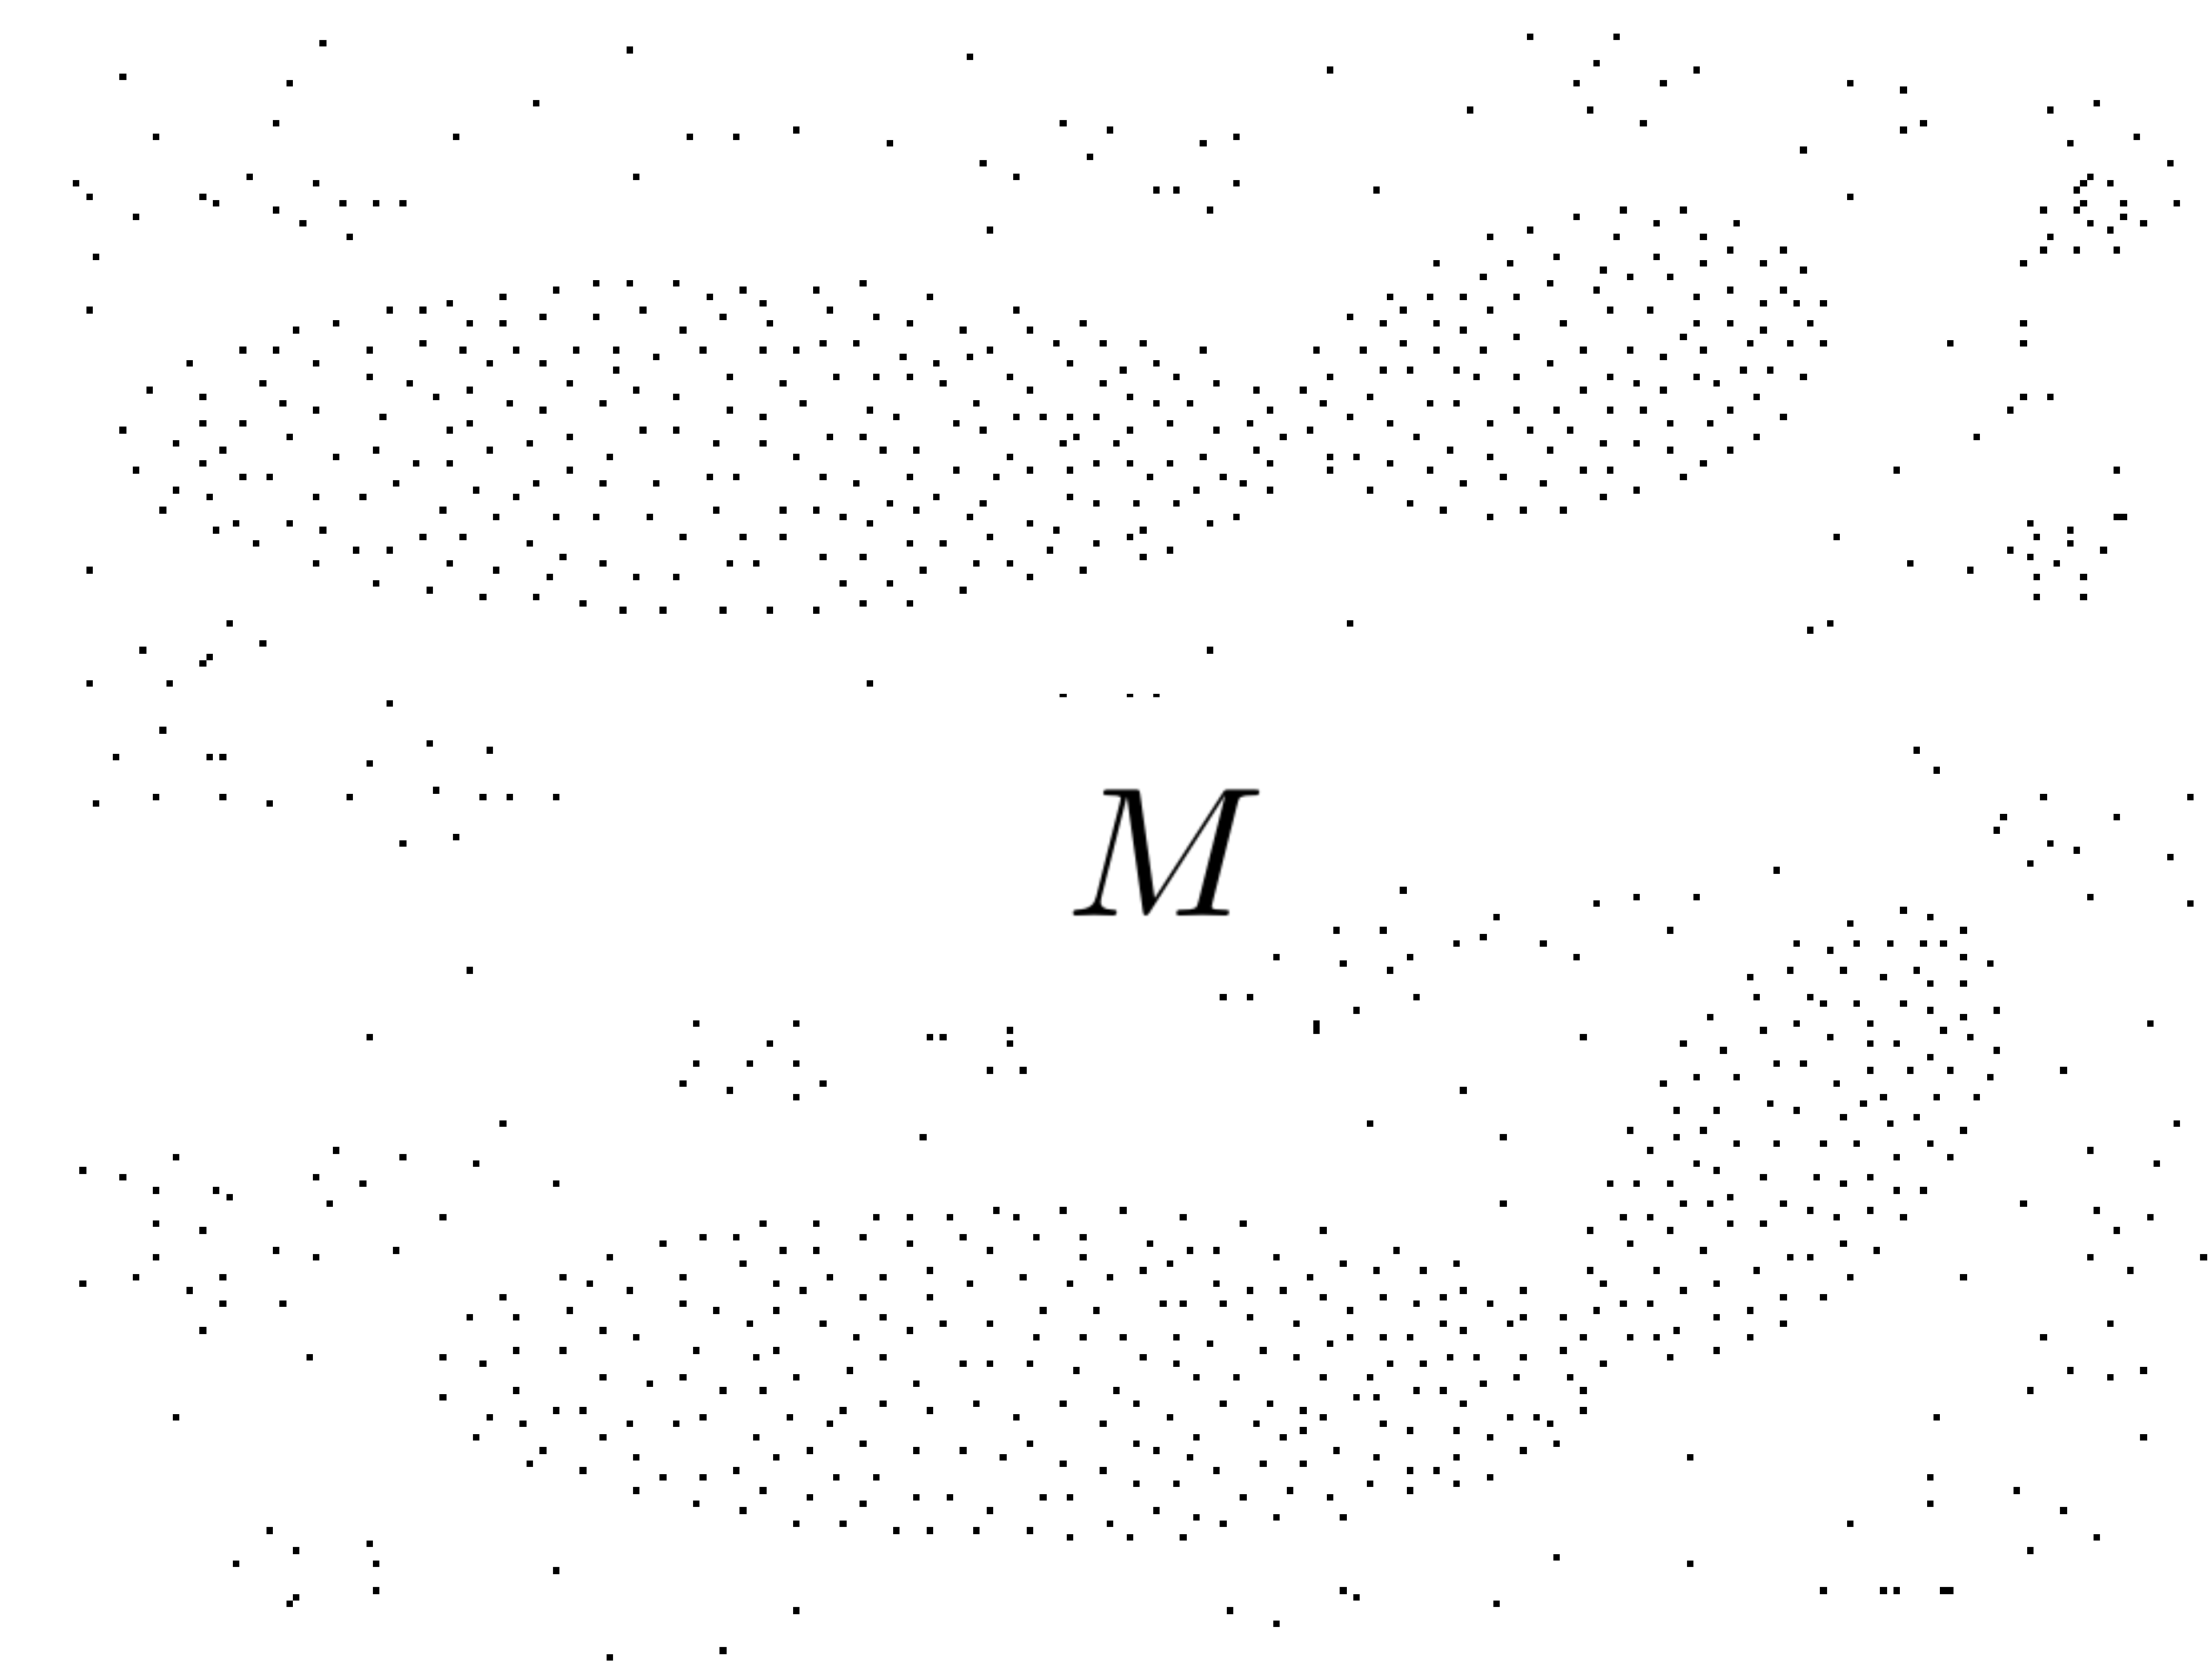
\includegraphics[width=0.45\textwidth]{pc_2parts_Noise}} &		% JPEG file
		\fbox{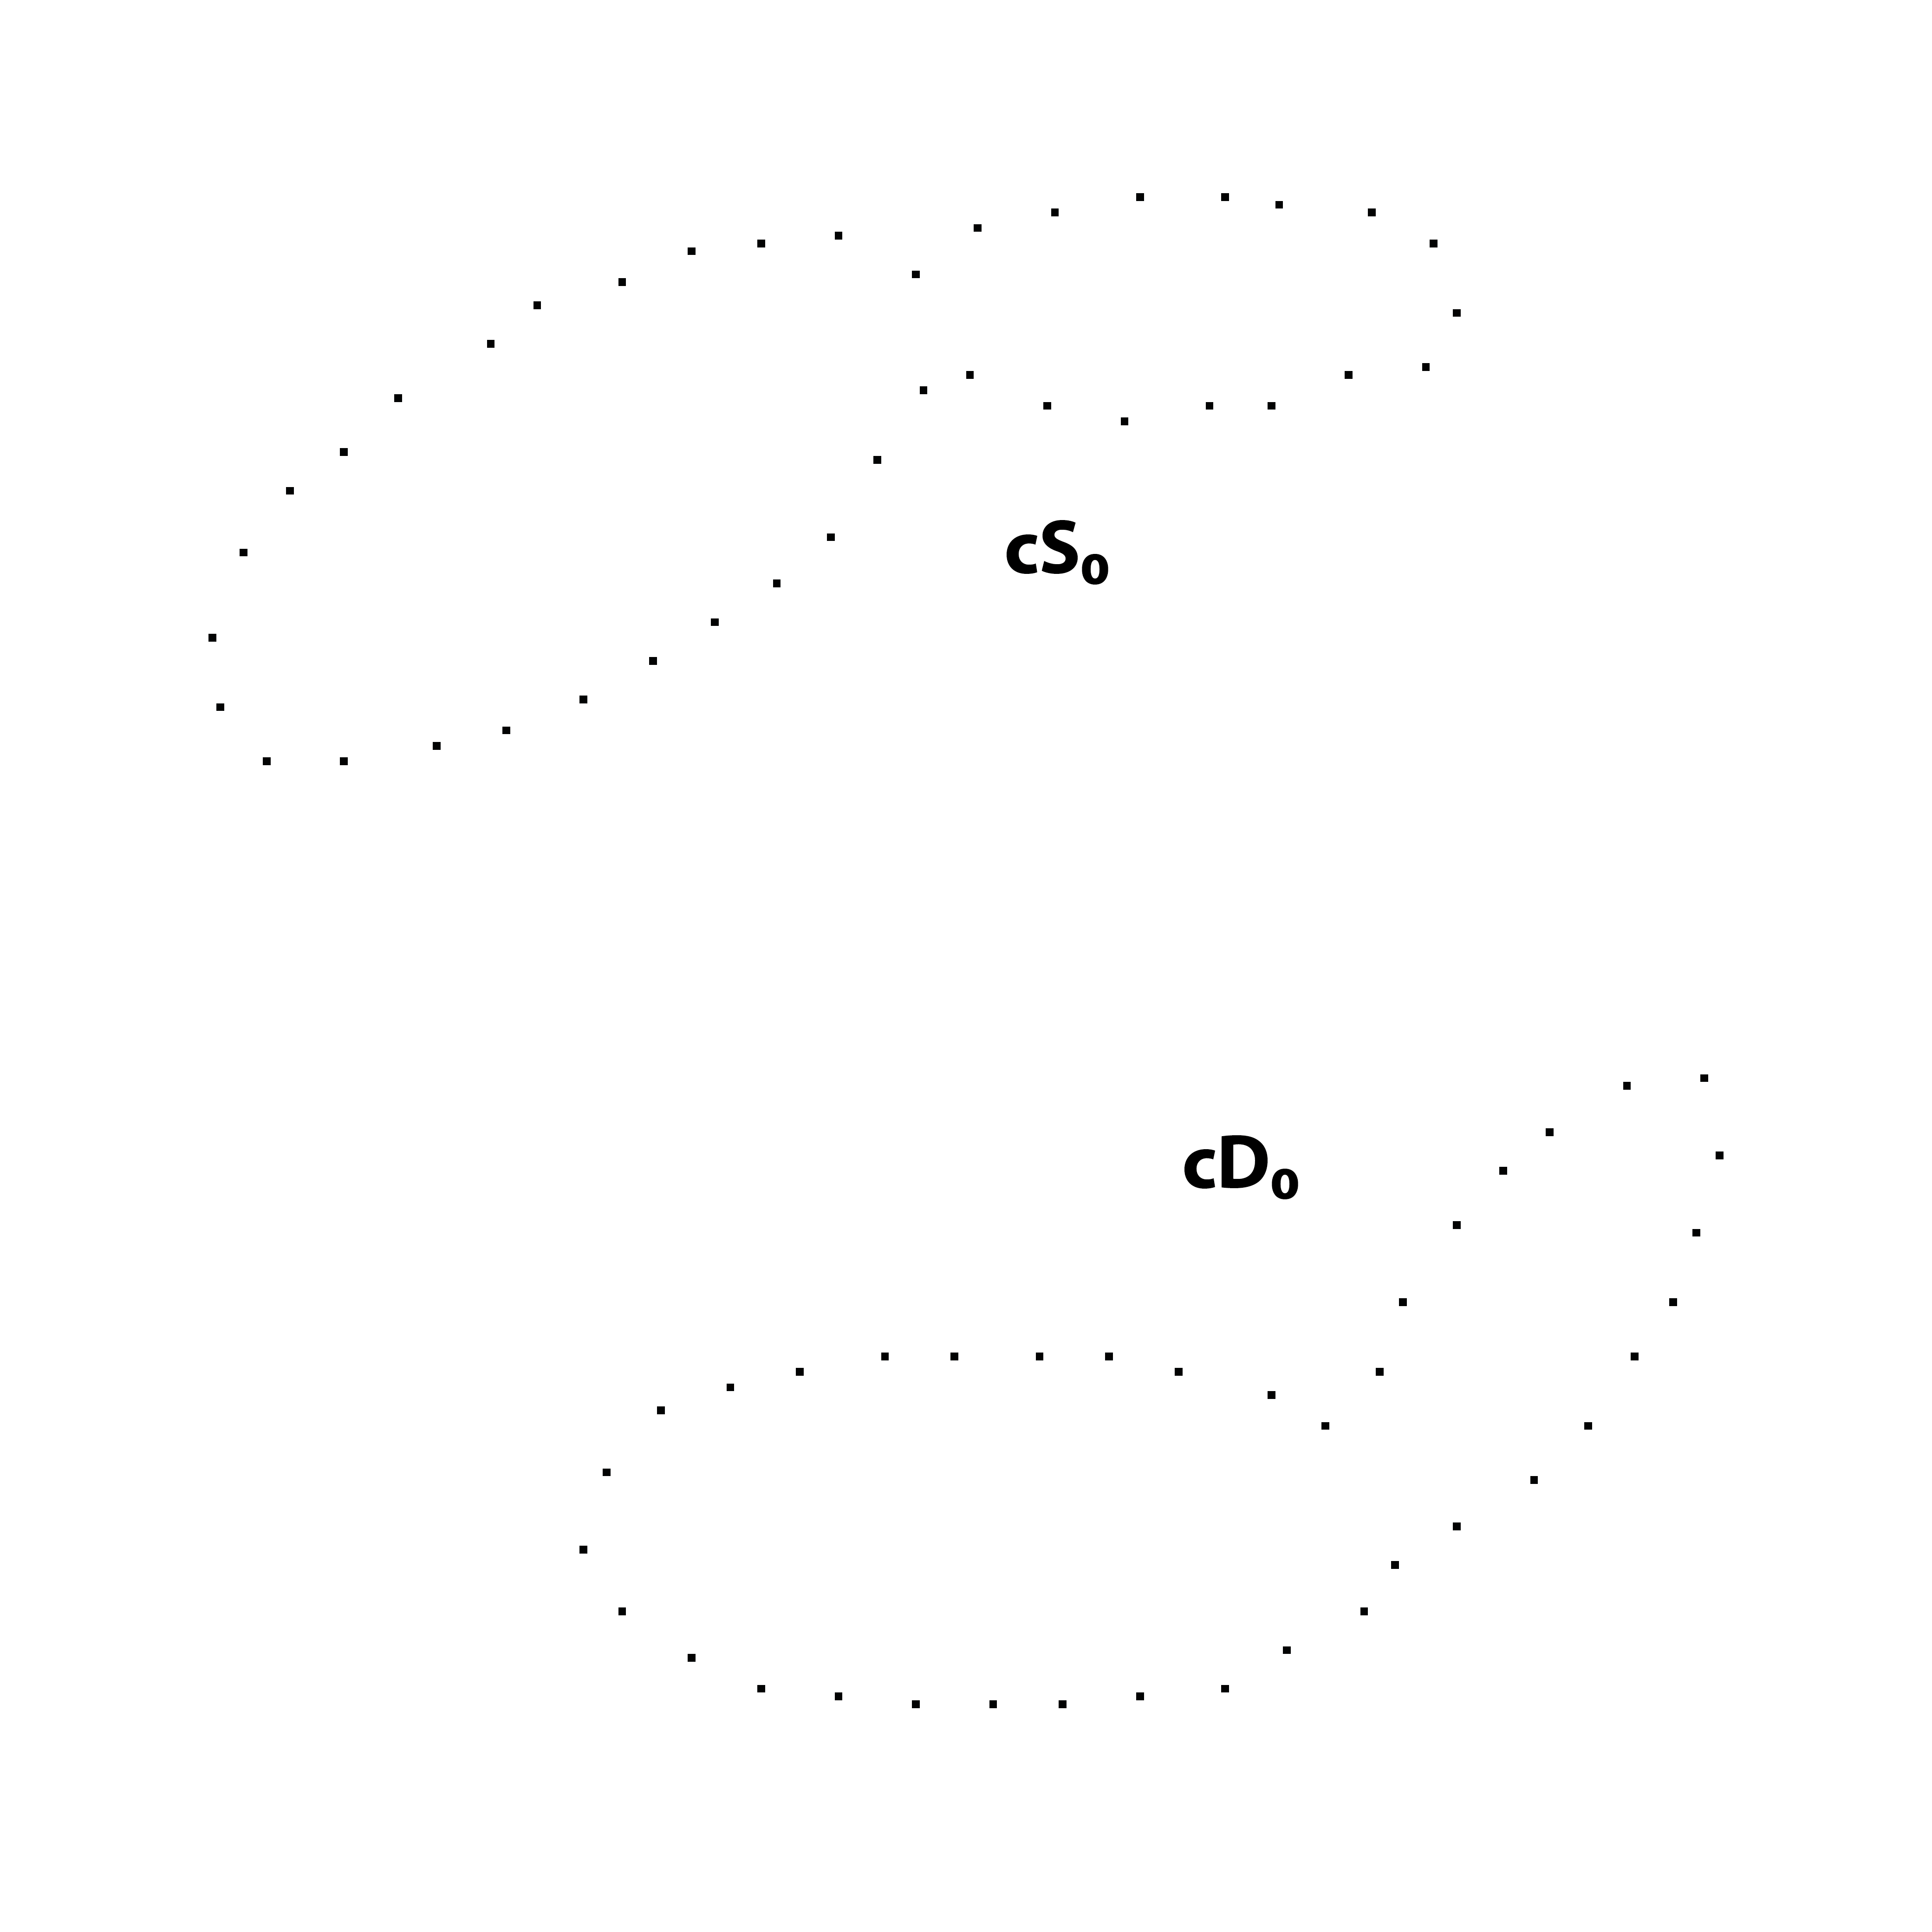
\includegraphics[width=0.45\textwidth]{pc_2parts_noNoise}} 
		\\	% PNG file
		(a) & (b) 
	\end{tabular}
	\caption{Taking a mesh $M$ in two different poses as input (a), removing noise of the input point clouds (b) to achieve the input clusters $C_{1,0}$ and $C_{2,0}$.} 
	\label{fig:pc_2parts}
\end{figure}

\subsection{Subdividing into clusters}

As a next step, the two main clusters $C_{1,0}$ and $C_{2,0}$ are taken as input for further computation steps. If the matching between two clusters does not succeed, they are both subdivided into two clusters. Otherwise, no subdividing is done. The whole procedure is repeated recursively for all clusters $\mathcal{C} = \{C_0, \ldots, C_m\}$ of $C_{1,0}$ and $C_{2,0}$ until all associated clusters of $C_{1,0}$ match the clusters of $C_{2,0}$.  

\subsubsection{Divider position}

To determine where to divide a cluster, it is taken advantage of the PCA (principal component analysis). As a first step the orientation $\theta$ of $C_{1,0}$ and $C_{2,0}$ are computed by calculating the central moments
%%
\begin{equation}
	\mu_{pq}(\mathcal{R}) = \sum_{(u,v)\in\mathcal{R}} (u - \bar{x})^p \cdot (v - \bar{y})^q
\end{equation}
%%
\begin{equation}
	\theta(\mathcal{R}) = \frac{1}{2} \tan^{-1} \left(\frac{2\cdot \mu_{11}(\mathcal{R})}{\mu_{20}(\mathcal{R}) - \mu_{02}(\mathcal{R})}\right)
\end{equation}
for each point cloud.	
The divider positions are determined by computing the principal axes $p_{1,0}$ and $p_{2,0}$ through the centroids and taking the perpendicular secondary axes $s_{1,0}$ and $s_{2,0}$ through the centroids (see figure \ref{fig:dc_axes_2p}). The secondary axes divide $C_{1,0}$ and $C_{2,0}$ into the sub clusters $C_{1,1}$ and $C_{1,2}$ as well as $C_{2,1}$ and $C_{2,2}$.

\begin{figure}
	\centering
	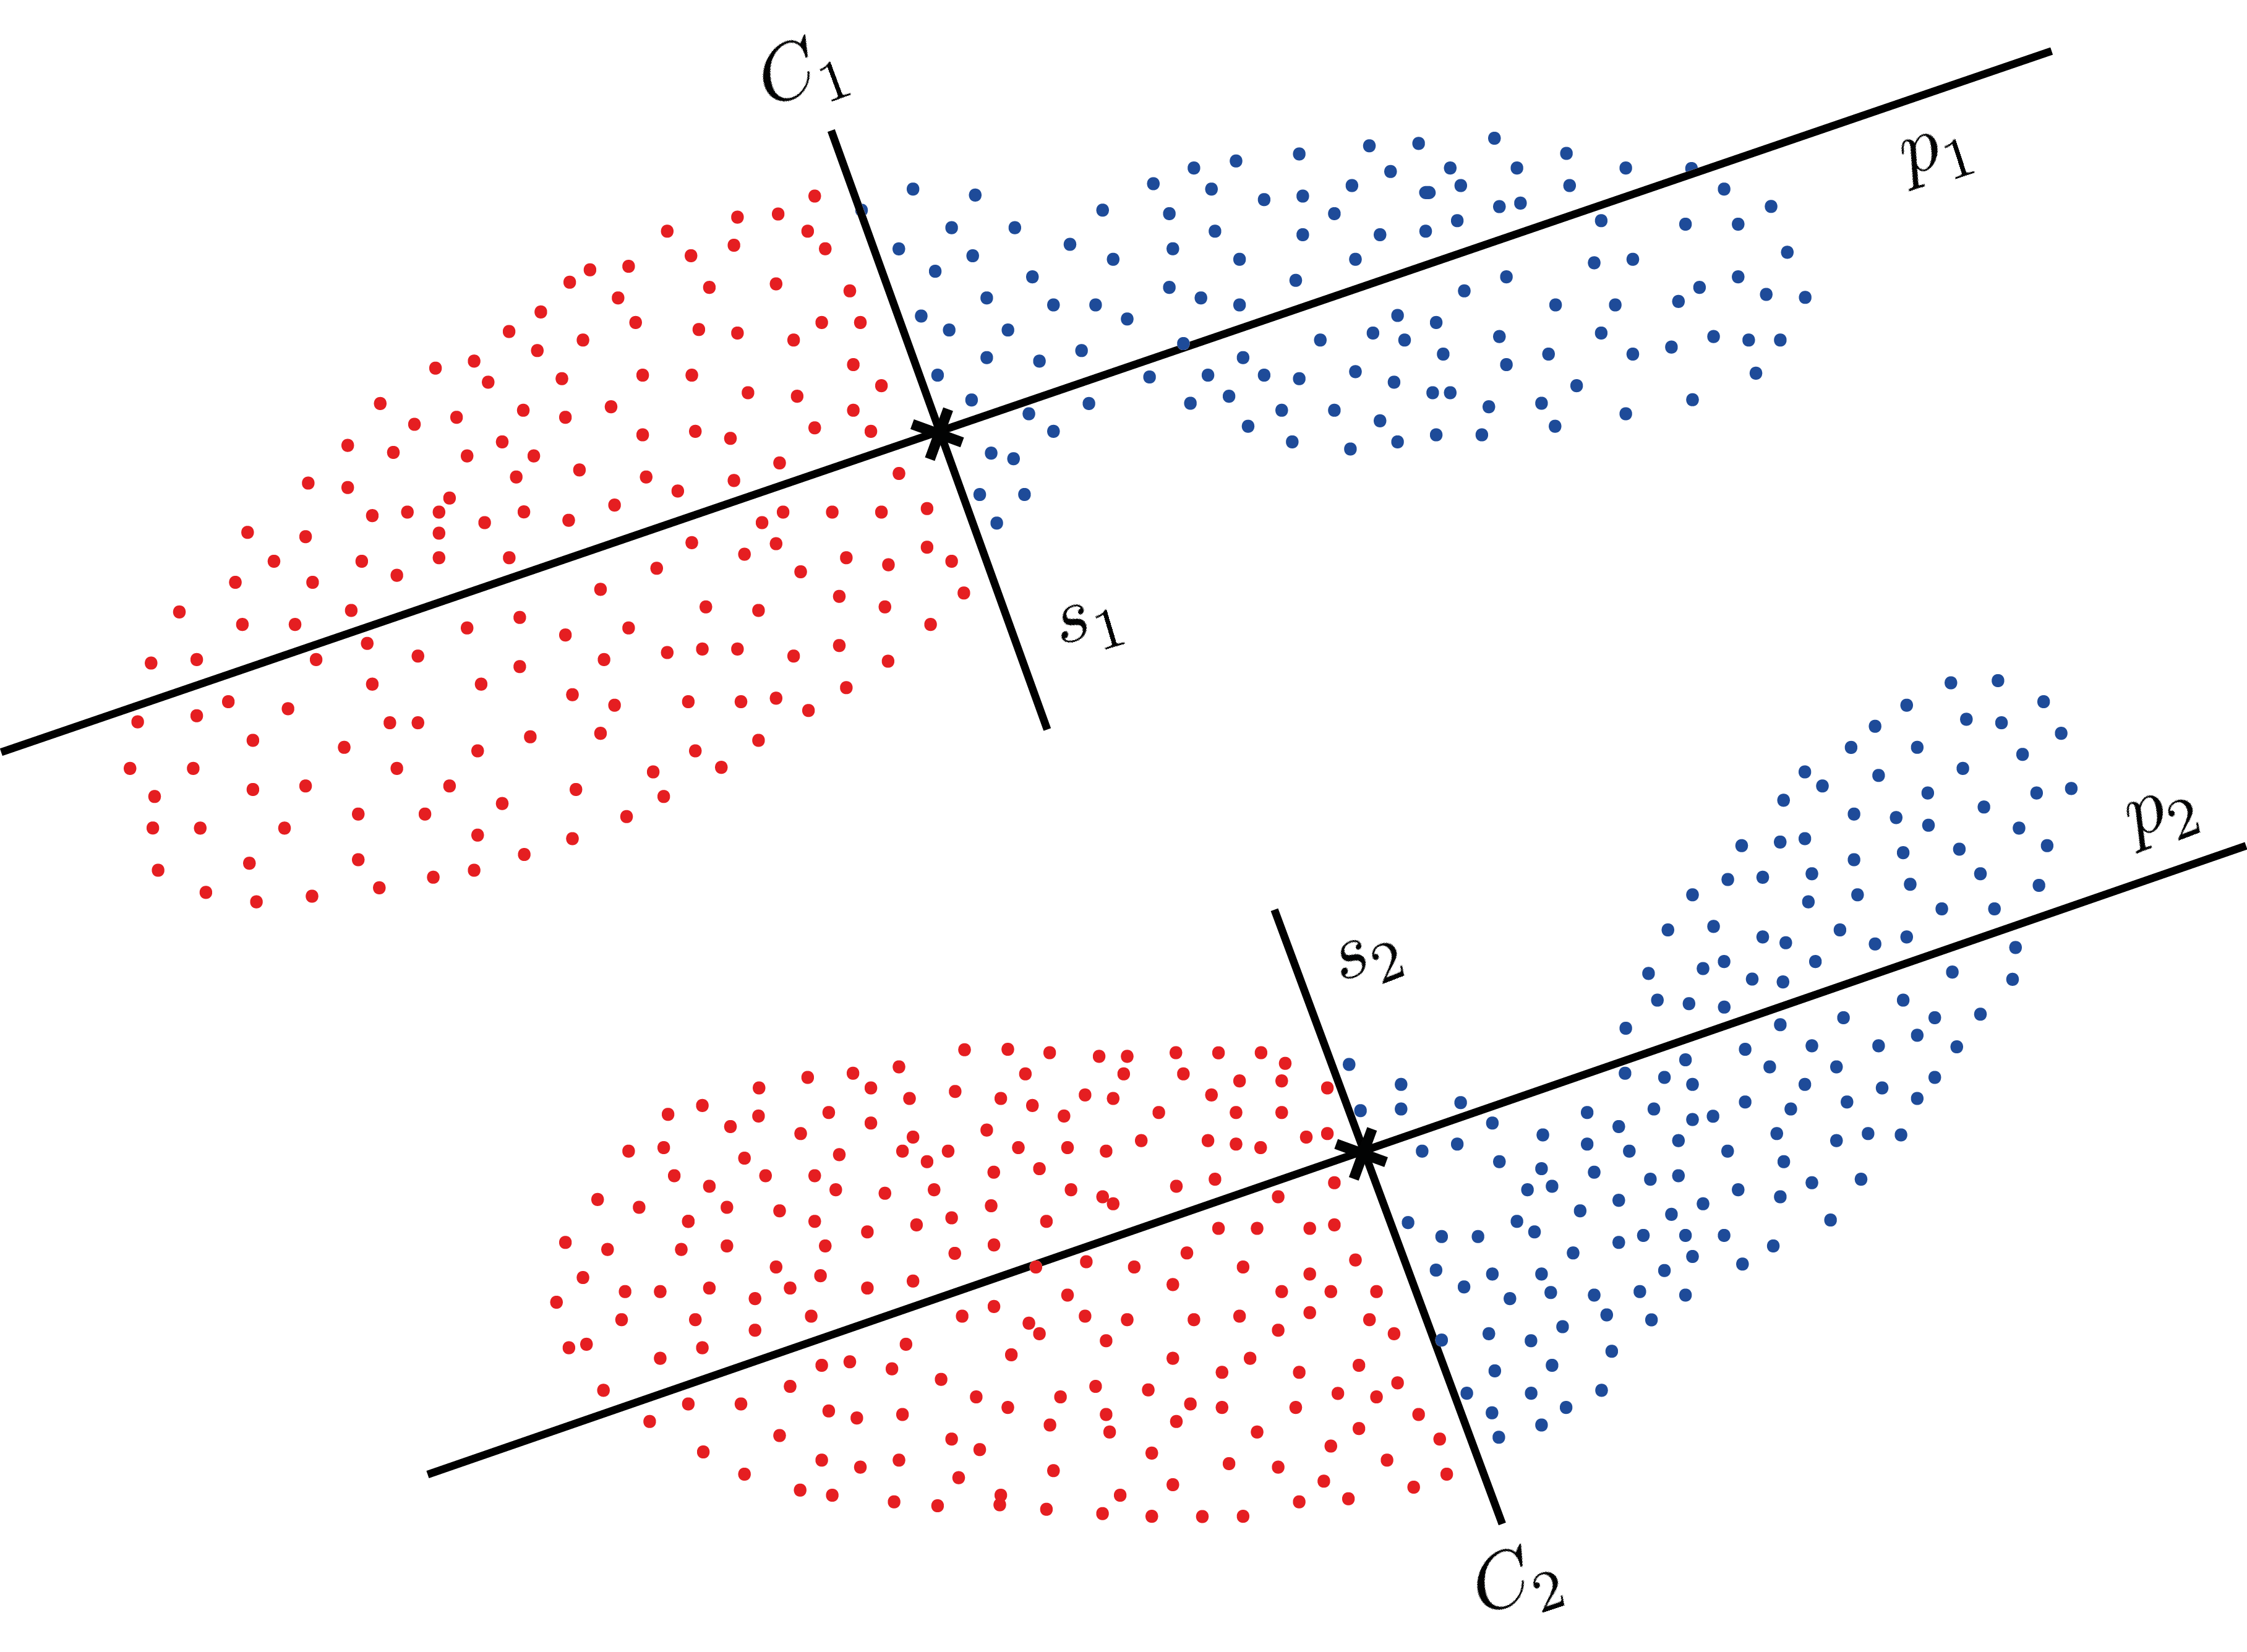
\includegraphics[width=0.8\linewidth]{illustration_axes}
	\caption{Subdividing $C_{1,0}$ and $C_{2,0}$ into two sub clusters by computing the secondary axes $s_{1,0}$ and $s_{2,0}$ perpendicular to $p_{1,0}$ and $p_{2,0}$ through the centroids.}
	\label{fig:dc_axes_2p}
\end{figure}

\subsubsection{Declaring the matching condition between two clusters}

By applying the ICP and the nearest neighbor approach on two associated clusters $C_{1,0}$ and $C_{2,0}$, a certain matching error $e$ is computed between the cluster points $ C_p =  \{ p_0, \ldots, p_m\}$ and the associated points $ C_q =  \{ q_0, \ldots, q_m\}$. To eliminate the dependency between the matching error and the number of cluster points $m$, the average error per point $C_p, C_q$
%
\begin{equation}
	e_{\mathrm{avg}(C_p, C_q)} = \frac{1}{| C_p |} \cdot \displaystyle\sum_{i=0}^{m}\| \boldsymbol{p}_i - \boldsymbol{q}_i\|^2
\end{equation}
%
is computed, assuming that the two clusters $C_p$ and $C_q$ contain the same number of cluster points $m$. In case of different point amounts, the segmentation needs to be carried out that clusters contain the same number of points. Alternatively, extra points are not considered in the error amount calculation. To declare when two clusters match, it is quite essential to determine an appropriate threshold $\tau$ for the maximum distance $d(p_0, q_0)$ between two associated points $p_0$ and $q_0$. In case of being overvalued, clusters are more likely to match which could result in insufficient subdividing. On the other hand, the clusters are difficult to be matched, which will result in further subdividing and the detection of too many rigid parts. The two clusters $C_p$ and $C_q$ are matching, if $e_{avg} < \tau$.

\subsubsection{Cluster tree}
\label{tree}

The subdividing of the clusters $C_{1,0}$ and $C_{2,0}$ is realized by a depth-first approach in a tree. Consequently, $C_{1,0}$ and $C_{2,0}$ are subdivided from the left to the right. A node $N$ of the tree contains two related clusters $C_{1,i}$ and $C_{2,i}$ and in case of subdividing them, a Node \textit{left}, containing the subdivided clusters $C_{1,i+1}$ and $C_{2,i+1}$, as well as a Node \textit{right}, containing the subdivided clusters $C_{1,i+2}$ and $C_{2,i+2}$. If two associated clusters $C_{1,i}$ and $C_{2,i}$ in a Node $N_i$ match, no further subdividing is performed. The resulting leaves of the tree are stored as matching clusters $\mathcal{C}_l = \{C_{l1,0},C_{l2,0}\ldots,C_{l1,m},C_{l2,m}\}$ (see figure \ref{fig:illustrationTree}). By applying the depth-first approach, the neighboring clusters in the list are also neighboring clusters in the main clusters $C_{1,0}$ and $C_{2,0}$.  As a result, in the following steps the skeleton structure from an object can be extracted, where parts are connected by joints.

\begin{figure}
	\centering
	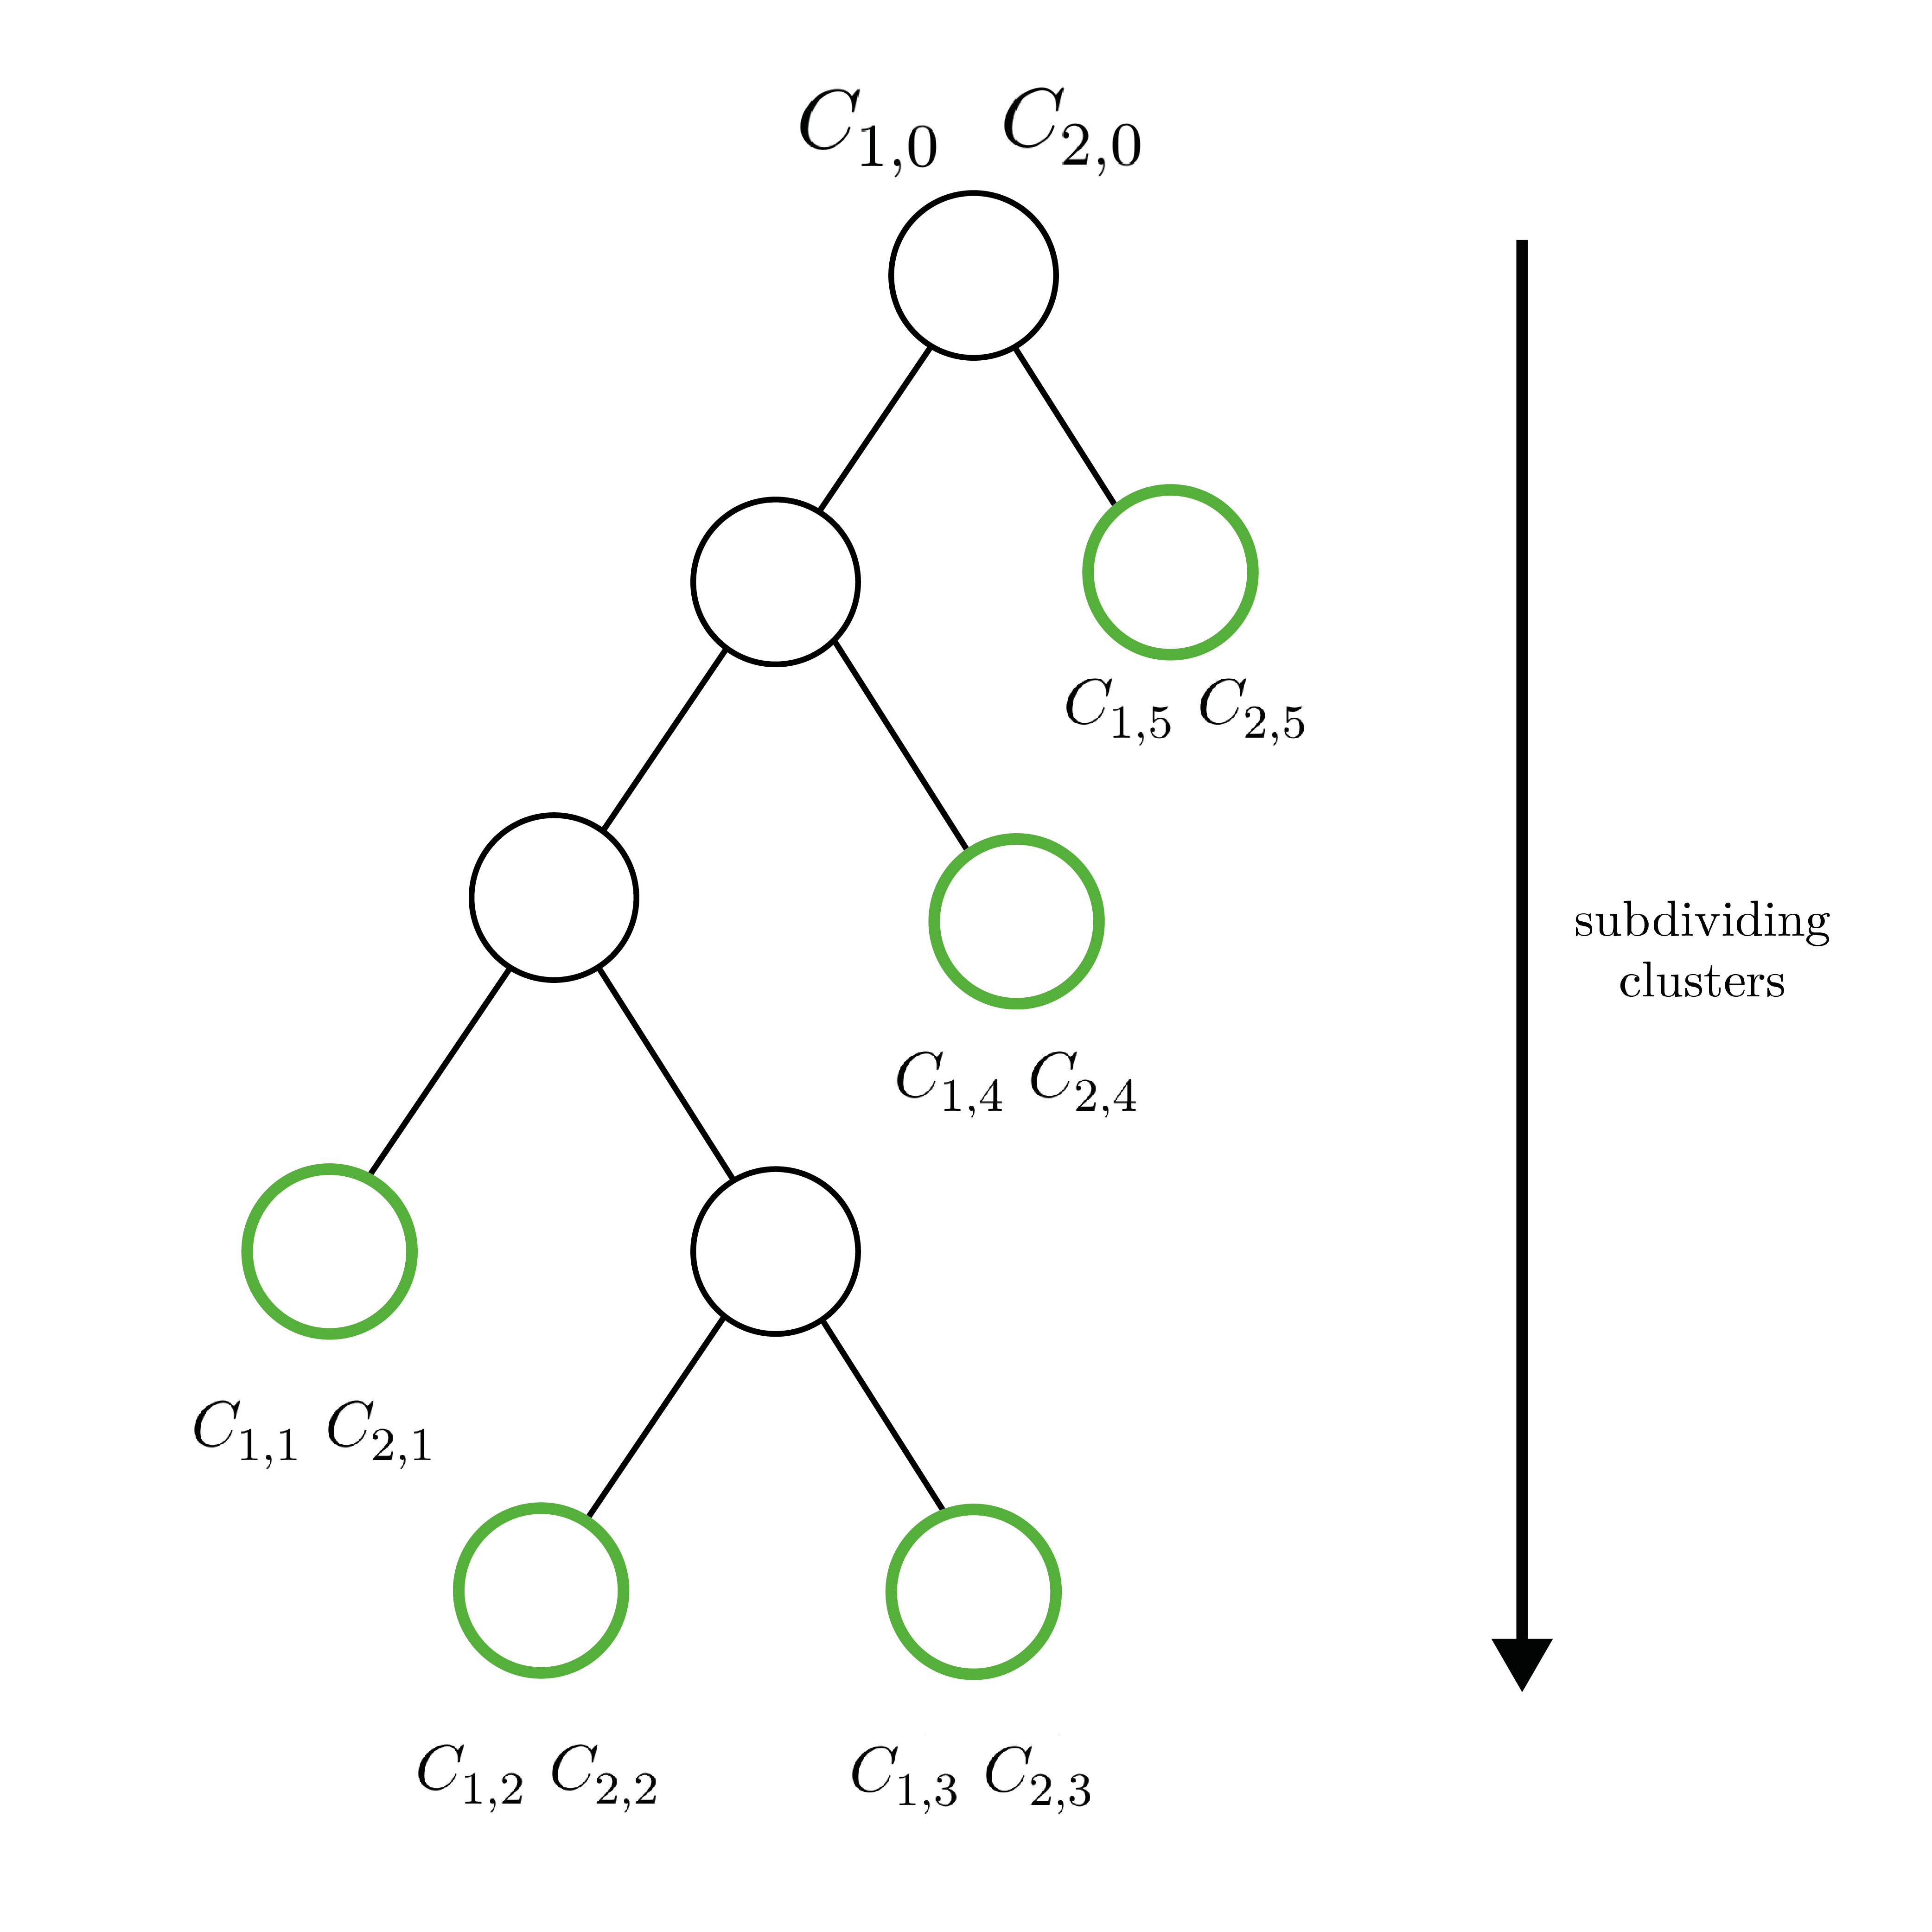
\includegraphics[width=0.7\linewidth]{IllustrationTree}
	\caption{Subdividing of $C_{1,0}$ and $C_{2,0}$ into matching clusters by the depth-first approach. The Subdividing terminates if all sub clusters of $C_{1,0}$ and $C_{2,0}$ match when applying the ICP.}
	\label{fig:illustrationTree}
\end{figure}

\subsection{Merging neighboring clusters to rigid parts}

As a next step, neighboring clusters from $\mathcal{C}_l$ are iteratively merged and subsequently verified to still match. This process is required to rejoin, if necessary, detected sub clusters to the rigid parts of the object. This is the case, if a rigid part was subdivided during the segmentation process. The merging initiates with the first clusters $C_{l1,0}$, $C_{l2,0}$ and its adjacent cluster $C_{l1,1},C_{l2,1}$. If the resulting merged clusters $C_{r1,0}$, $C_{r2,0}$ can be matched, the merging proceeds with $C_{r1,0}$, $C_{r2,0}$ and the adjacent cluster $C_{l1,2},C_{l2,2}$. If not, the merging is not executed and $C_{l1,0}$, $C_{l2,0}$ are stored in a list of resulting clusters $C_r$. The merging procedure then continues with $C_{l1,1},C_{l2,1}$. The process terminates if all clusters of $C_l$ are verified and consequently the clusters of $C_r$ are assigned to rigid parts $ \mathcal{P} =  \{P_1,\ldots,P_n\}$ (see figure \ref{fig:clusterChain}). 

\begin{figure}
	\centering
	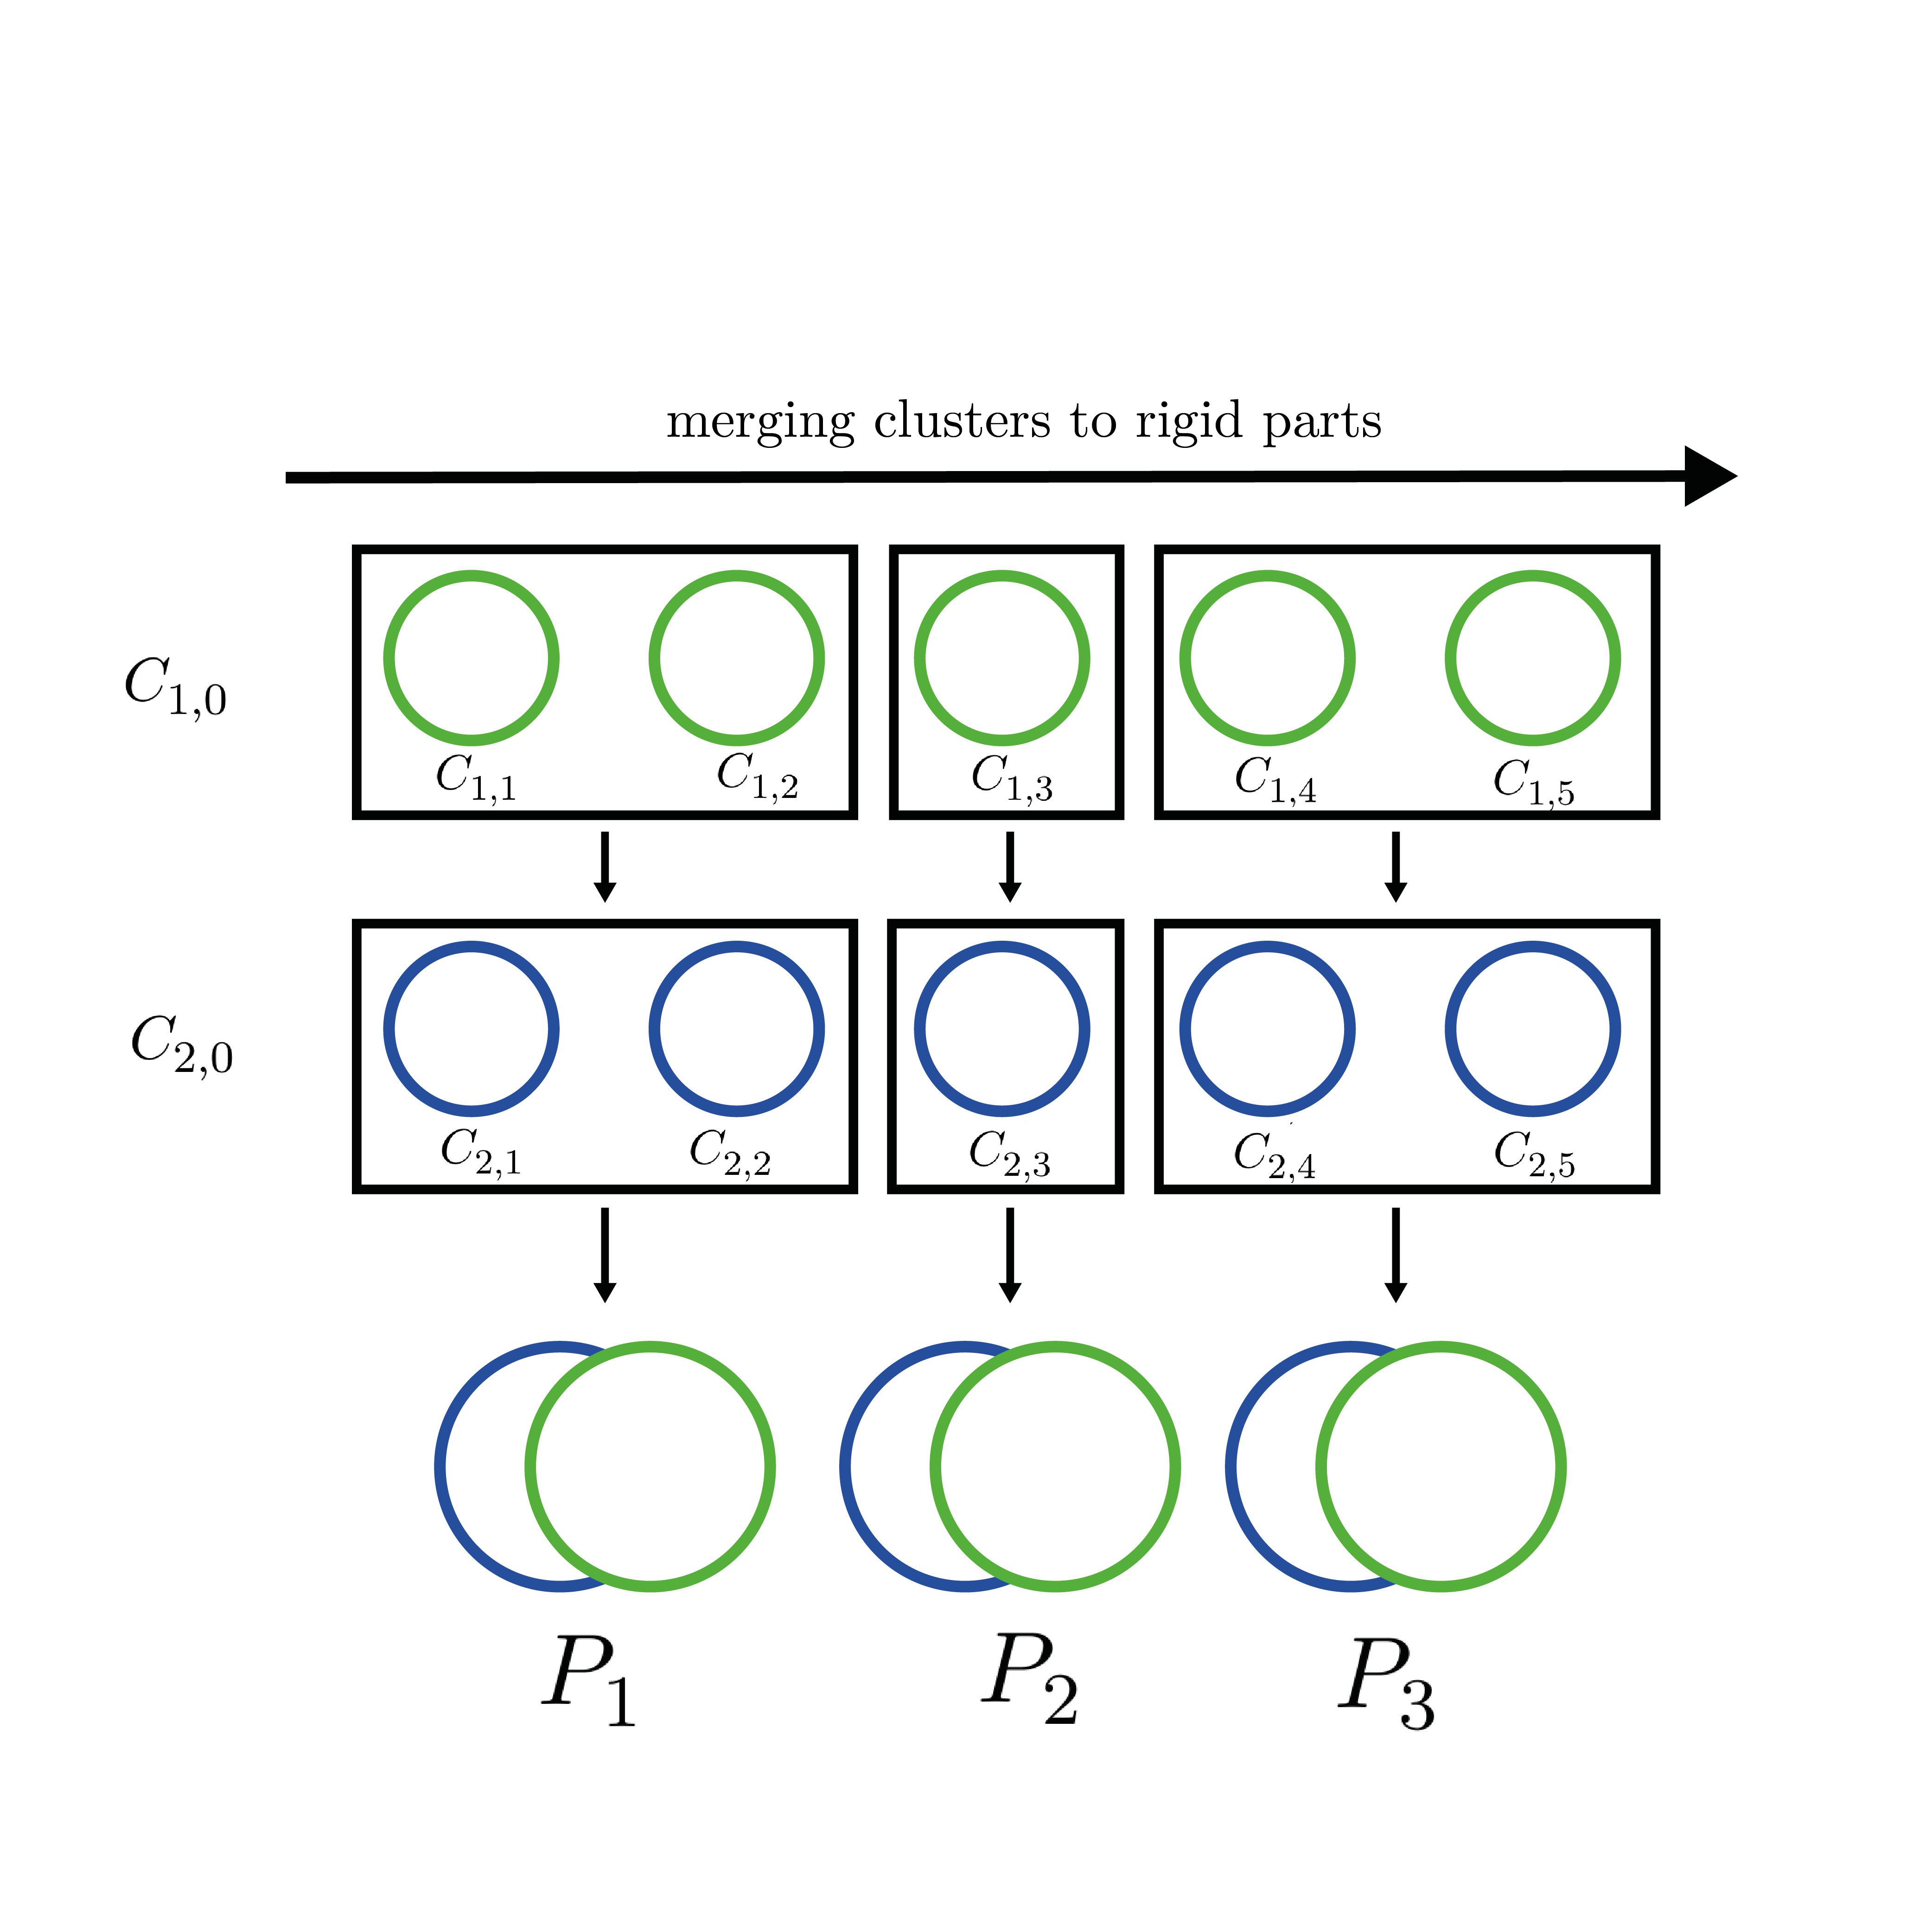
\includegraphics[width=0.7\linewidth]{ClusterChain}
	\caption{Detecting rigid parts of $C_{1,0}$ and $C_{2,0}$ by iteratively merging neighboring clusters of $C_l$ that merged clusters still match.}
	\label{fig:clusterChain}
\end{figure}

\subsection{Joint/skeleton estimation}

After detecting the rigid parts $\mathcal{P} =  \{ {P_1,....P_n}\}$, they are linked with joints.

\chapter{Implementation and Results}

My approach was implemented in Java, using ImageJ as processing library, to focus on implementing and testing the algorithm in 2D. Another implementation is planned in 3D with the PCL to bring the attention to segmentation and visualization in 3D. A class \texttt{Cluster} was implemented to store the cluster's points, its centroid, the orientation $\theta$ as well as the principal and secondary axes. For the subdividing, a \texttt{ClusterTree} was implemented to simultaneously divide the main clusters $C_{1,0}$ and $C_{2,0}$ into sub clusters (see algorithm \ref{subdividing}). Each node $N$ contains thereby two associated clusters $C_{1,i}$ and $C_{2,i}$. For the clustering and merging of clusters a \texttt{List<Clusters>} was used to dynamically add and remove Clusters. Furthermore, a class \texttt{ICP} was created, which takes two clusters to be matched as input.
\begin{algorithm}[tbp]
	\caption{Recursive subdividing of two main clusters $C_{1,0}$ and $C_{2,0}$ into matching sub clusters. The ICP is applied on two clusters to verify them to match.}
	\label{alg:clustering}
	
	\begin{algorithmic}[1]     % [1] = all lines are numbered
		\label{subdividing}
		\Procedure{Subdivide}{$currentNode$} 
		
		\If {\Call{match}{$currentNode[0]$, $currentNode[1]$}}
		\Comment{Apply ICP on two clusters}
		\State $subclusters.add(currentNode)$
		
		\Else
		\State \Call{Split}{$currentNode$}
		\Comment{Splits a cluster into a left and right side}
		\State \Call{Subdivide}{$currentNode.left$}
		\State \Call{Subdivide}{$currentNode.right$}
		
		\EndIf
		\\
		
		\EndProcedure	
		
		
		\Procedure{Main}{$C_{1,0}$, $C_{2,0}$}
		\Statex Returns the subdivided input clusters if all are matching.
		\Comment{take main clusters as input}
		
		\State $List<cluster> subclusters$
		\State $root \gets C_{1,0}, C_{2,0}$
		\State $root.left \gets null$
		\State $root.right \gets null$
		
		\Call{Subdivide}{$root$}
		
		\State\Return $\mathit{subclusters}$
		
		\EndProcedure
	\end{algorithmic}
\end{algorithm}

\section{Intermediate results}

At first, the implementation was tested on two point clouds of an articulated object with only two rigid parts. The segmentation results are directly dependent on the matching error threshold $\tau$ which can bee seen on table \ref{table:segmentation_results}. The higher the threshold $\tau$, the less clusters and subsequently rigid parts can be detected, as two clusters are more likely to match and are not further subdivided. The lower $\tau$, the more clusters and rigid parts will be detected, as clusters require further subdividing in order to match. Figure \ref{fig:2rigidParts} and figure \ref{fig:3rigidParts} show the clustering and rigid part detection of two simple objects, in regard to their rigid parts linked like a chain. For those objects, with a threshold $\tau = 5$ the right number of rigid parts is detected. However, the segmentation position does not correspond to the actual joint of $C_{1,0}$ and $C_{2,0}$. The reason is, that the average error $e_{avg}$ is computed without any weighting of points. Especially points located near a joint need to be treated cautiously. Figure \ref{fig:4rigidParts} shows a more complex object.
%%
\begin{table}
	\centering\small
	\begin{tabular}{ |c|c|c|c| } 
		\hline
		Rigid parts & $\tau$ & detected clusters & detected rigid parts \\
		\hline
		& 3 & 21 & 14 \\ 
		2& 5 & 3 & 2 \\
		& 7 & 2 & 2 \\
		\hline
		& 4 & 38 & 31 \\ 
		3 & 6 & 4 & 3 \\
		& 8 & 3 & 3 \\
		\hline
		& 6 & 35 & 26 \\ 
		4 & 7 & 3 & 3 \\
		& 8 & 3 & 3 \\
		\hline
	\end{tabular}
	\caption{Segmentation results}
	\label{table:segmentation_results}
\end{table}
%%
\begin{figure}
	\centering\small
	\begin{tabular}{@{}c@{\hspace{2mm}}c@{}} % mittlerer Abstand = 12mm
		\fbox{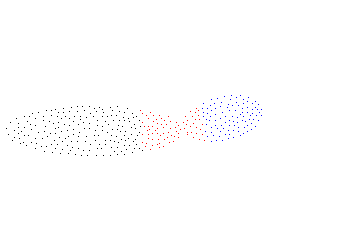
\includegraphics[width=.40\textwidth]{results/2_1parts_clusters_2th}} &
		\fbox{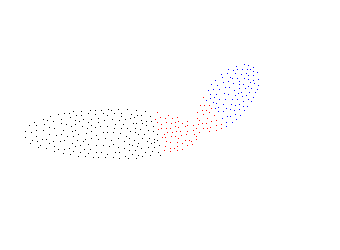
\includegraphics[width=.40\textwidth]{results/2_2parts_clusters_2th}} 
		\\
		(a) & (b)
		\\[4pt]	%vertical extra spacing (4 points)
		\fbox{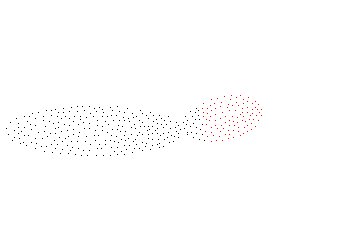
\includegraphics[width=.40\textwidth]{results/2_1parts_rigidParts_2th}} &
		\fbox{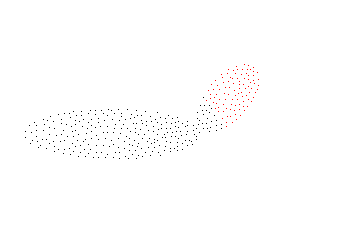
\includegraphics[width=.40\textwidth]{results/2_2parts_rigidParts_2th}} 
		\\
		(c) & (d)
	\end{tabular}
	\caption{Taking a Mesh $M$ in two poses with only two rigid parts as input, with a threshold $\tau = 5$, 3 clusters are detected in $C_{1,0}$~(a) and $C_{2,0}$~(b),
		which results in 2 rigid parts in $C_{1,0}$~(c) and $C_{2,0}$~(d).}
	\label{fig:2rigidParts}
\end{figure}
%%
\begin{figure}
	\centering\small
	\begin{tabular}{@{}c@{\hspace{2mm}}c@{}} % mittlerer Abstand = 12mm
		\fbox{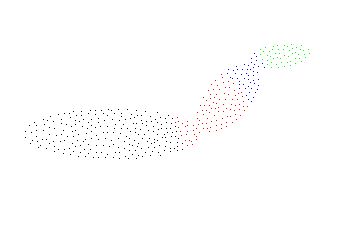
\includegraphics[width=.40\textwidth]{results/3_1parts_clusters_2th}} &
		\fbox{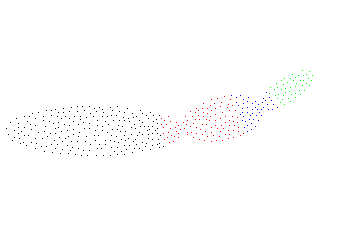
\includegraphics[width=.40\textwidth]{results/3_2parts_clusters_2th}} 
		\\
		(a) & (b)
		\\[4pt]	%vertical extra spacing (4 points)
		\fbox{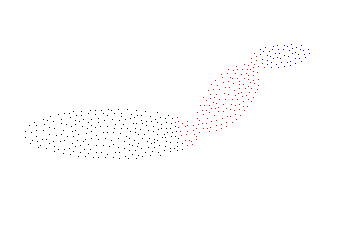
\includegraphics[width=.40\textwidth]{results/3_1parts_rigidParts_2th}} &
		\fbox{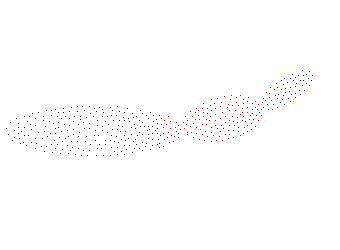
\includegraphics[width=.40\textwidth]{results/3_2parts_rigidParts_2th}} 
		\\
		(c) & (d)
	\end{tabular}
	\caption{Taking a Mesh $M$ in two poses with three rigid parts as an input, with a threshold $\tau = 6$, 4 clusters are detected in $C_{1,0}$~(a) and $C_{2,0}$~(b),
		which results in 3 rigid parts in $C_{1,0}$~(c) and $C_{2,0}$~(d).}
	\label{fig:3rigidParts}
\end{figure}
The segmentation into rigid parts is also apparent, when visualizing the point registration between $C_{1,0}$ and $C_{2,0}$ (see figure \ref{fig:ICPResults}). Two associated points from $C_{1,0}$ and $C_{2,0}$ are thereby linked with green lines. Comparing the registration results before and after a segmentation into rigid parts clearly shows, that the registration of rigid parts with the ICP results in a lower matching error $e$.
%%	
\begin{figure}[H]
	\centering\small
	\begin{tabular}{cc}
		\fbox{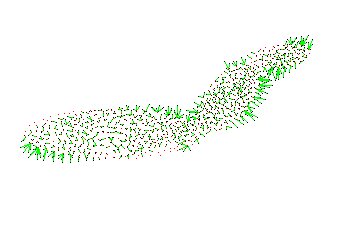
\includegraphics[width=0.45\textwidth]{results/non-rigid_3parts_associations}} &		% JPEG file
		\fbox{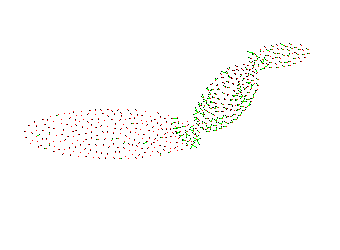
\includegraphics[width=0.45\textwidth]{results/rigid_3parts_associations}} 
		\\	% PNG file
		(a) & (b) 
	\end{tabular}
	\caption{Registration of $C_{1,0}$ and $C_{2,0}$ before the segmentation into rigid parts (a) and after the segmentation.} 
	\label{fig:ICPResults}
\end{figure}
%%		
In case of a more complex object, the simple segmentation algorithm fails. Although varying threshold $\tau$ for the matching, there are either too many or few rigid parts detected. When using $\tau = 7$ (see figure \ref{fig:4rigidPartsHighTH}) only 3 clusters and rigid parts can be detected. By decreasing $\tau$ to 6 (see Figure \ref{fig:4rigidParts}), further subdividing is done, which leads to a too high number of rigid parts and clusters.
%%
\begin{figure}[H]
	\centering\small
	\begin{tabular}{cc}
		\fbox{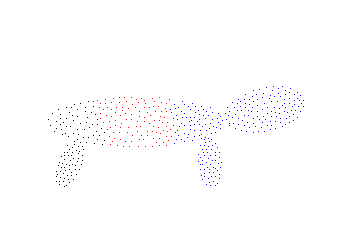
\includegraphics[width=0.45\textwidth]{results/4_1parts_clusters_rigidParts_7th}} &		% JPEG file
		\fbox{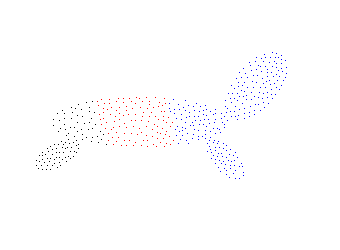
\includegraphics[width=0.45\textwidth]{results/4_2parts_clusters_rigidParts_7th}} 
		\\	% PNG file
		(a) & (b) 
	\end{tabular}
	\caption{Taking a more complex Mesh $M$ in two poses with four rigid parts as an input, with a threshold $\tau = 7$, 3 clusters and rigid parts can be detected in $C_{1,0}$~(a) and $C_{2,0}$~(b).} 
	\label{fig:4rigidPartsHighTH}
\end{figure}
\begin{figure}[H]
	\centering\small
	\begin{tabular}{@{}c@{\hspace{2mm}}c@{}} % mittlerer Abstand = 12mm
		\fbox{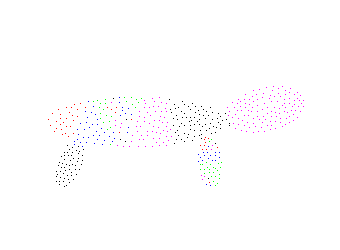
\includegraphics[width=.40\textwidth]{results/4_2parts_clusters_6th}} &
		\fbox{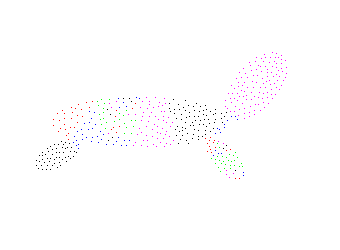
\includegraphics[width=.40\textwidth]{results/4_1parts_clusters_6th}} 
		\\
		(a) & (b)
		\\[4pt]	%vertical extra spacing (4 points)
		\fbox{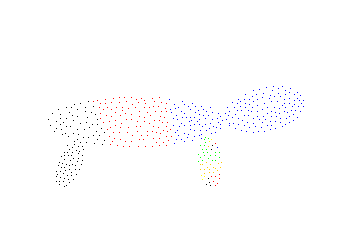
\includegraphics[width=.40\textwidth]{results/4_1parts_rigidParts_6th}} &
		\fbox{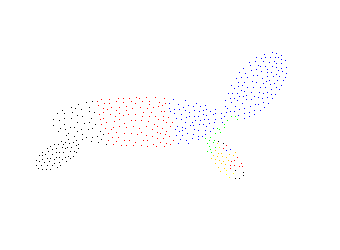
\includegraphics[width=.40\textwidth]{results/4_2parts_rigidParts_6th}} 
		\\
		(c) & (d)
	\end{tabular}
	\caption{Taking a more complex Mesh $M$ in two poses with four rigid parts as an input, with a threshold $\tau = 6$ , 35 clusters are detected in $C_{1,0}$~(a) and $C_{2,0}$~(b),
		which results in 26 rigid parts in $C_{1,0}$~(c) and $C_{2,0}$~(d).}
	\label{fig:4rigidParts}
\end{figure}	
The algorithm generally works for simple objects, in which the rigid parts are linked like a chain. Still, the segmentation location is not accurate, which might be disposed by introducing weights to points located near a joint. For more complex object with a skeleton structure, e.g. a human, where one rigid part is linked to more than two rigid parts, this simple implementation fails. In this case, another approach has to be found, as a skeleton structure is more complex to extract than a simple chain structure.

\section{Possible Improvements}

\subsection{LRP as initial alignment}
As the segmentation algorithm fails for objects with a skeleton structure, the LRP algorithm might be pursued as an initial step (see section \ref{sec:LRP}). Thereby the largest rigid part is assumed to be the part with most joints to other rigid parts. 

\subsection{Matching error}
Another improvement possibility would be to ensure that during the ICP procedure each point only has one nearest neighbor and also considering the case, that there are not always the same amount of points in two clusters. Furthermore, weights should be added to the points, especially points located near a joint should be treated cautiously. 

\subsection{Checking for multiple clusters}
A similar approach to the LRP algorithm \cite{guo2016correspondence} would be the detection of multiple clusters by region growing, in case of sub dividing a cluster. The detected clusters are then treated individually.

\section{LRP}
\label{sec:LRP}
Instead of starting to subdivide the clusters $C_{1,0}$ and $C_{2,0}$ in each two sub clusters, as an initial step the largest rigid part is detected and recursively all other linked parts can be detected.

\subsection{Overview}
As an initial step, the LRP algorithm tries to find the most reliable correspondences, the so-called largest rigid part (LRP), subsequently all other parts are detected that are linked to the LRP. The initial alignment stage tries to find sparse correspondences between two point clouds by applying a single rigid transformation to detect the largest subsets of points in two point clouds. Starting from the LRP all other parts are detected recursively.
\subsection{Algorithm} 

\subsubsection{Finding the LRP}

The algorithm takes two point clouds $C_{1,0}$ and $C_{2,0}$ of the same object in different configurations as input.
The goal is to find a single rigid transformation $T_{init}$ for all points of $C_{1,0}$ to obtain potential corresponding points between $C_{1,0}$ and $C_{2,0}$. For that, local descriptors of $C_{1,0}$ and $C_{2,0}$ are computed. The requirement for a sparse correspondence between two points $\boldmath{p}_{1,i}$ and $\boldmath{p}_{2,i}$  is that they are \textit{reciprocal}, which means that the euclidean distance $d(\boldmath{p}_{1,i}, \boldmath{p}_{2,i})$ between them is the smallest in both directions. Some of the sparse correspondences are assumed to be wrong. Therefore, RANSAC is applied on the sparse correspondences  to estimate a rigid alignment that is supported by the largest number of points $n$ from $C_{1,0}$ and $C_{2,0}$. To assign the LRP in $C_{1,0}$ and $C_{2,0}$, the biggest point clusters $C_{1,1}$ and $C_{2,1}$ of the overlapping areas $\mathcal{C}_1 = \{C_{1,1}\ldots,C_{1,n}\}$ and  $\mathcal{C}_2 = \{C_{2,1}\ldots,C_{2,n}\}$ are detected. 


\subsubsection{Part discovery}

The remaining clusters from $C_{1,0}$ and $C_{2,0}$ that have not been registered yet are matched recursively by starting with clusters connected to already matched parts. As a first step, all matched parts are excluded from the input point clouds. Then, clusters of all remaining points are formed by region growing, taking into account that they are attached to already registered parts. The algorithm of finding the LRP is applied until all body parts have been discovered.